\section{Corrections}

When analyzing the data, there are several corrections that need to be made. These are due to various physical or systematic effects that took place during the experiment. These effects have been studied in order to determine a ``correction factor'' that can be applied to the data.

\subsection{Target Boiling}
\label{sec:boiling}

Reference Sheren and Natalie paper.

Localized heating from the beam causes changes to the gas density of the target. The target does not actually boil, but the standard nomenclature for a change in target density is "boiling". By modulating the gas density, the incident beam sees a variable target thickness. This in turn affects the yield calculation.

This effect scales with the current that is on the target. We make this correction run-by-run using the average current during beam-on time during the run. This method was chosen because the average current is near constant over the coarse of a single run and the effect is approximately linear for small deviations in current. It was found that the change in density settles very quickly, so it is unnecessary to take into account beam ramp-up after beam trips.

To determine the correction, a dedicated set of runs was taken with the Left HRS spectrometer at $16.8\degree$ and $3.1GeV$. The data was taken at varying currents in order to assess the affect of the beam current on the normalized yield. By applying nominal event cuts to this data, the normalized yield was calculated. 

To determine the density correction, the normalized yields were plotted versus the beam current for that measurement. The data was then fit with a quadratic polynomial. The fit was constrained to require a correction of $1$ (no correction) at a current of $0 \mu A$.

\begin{figure}
	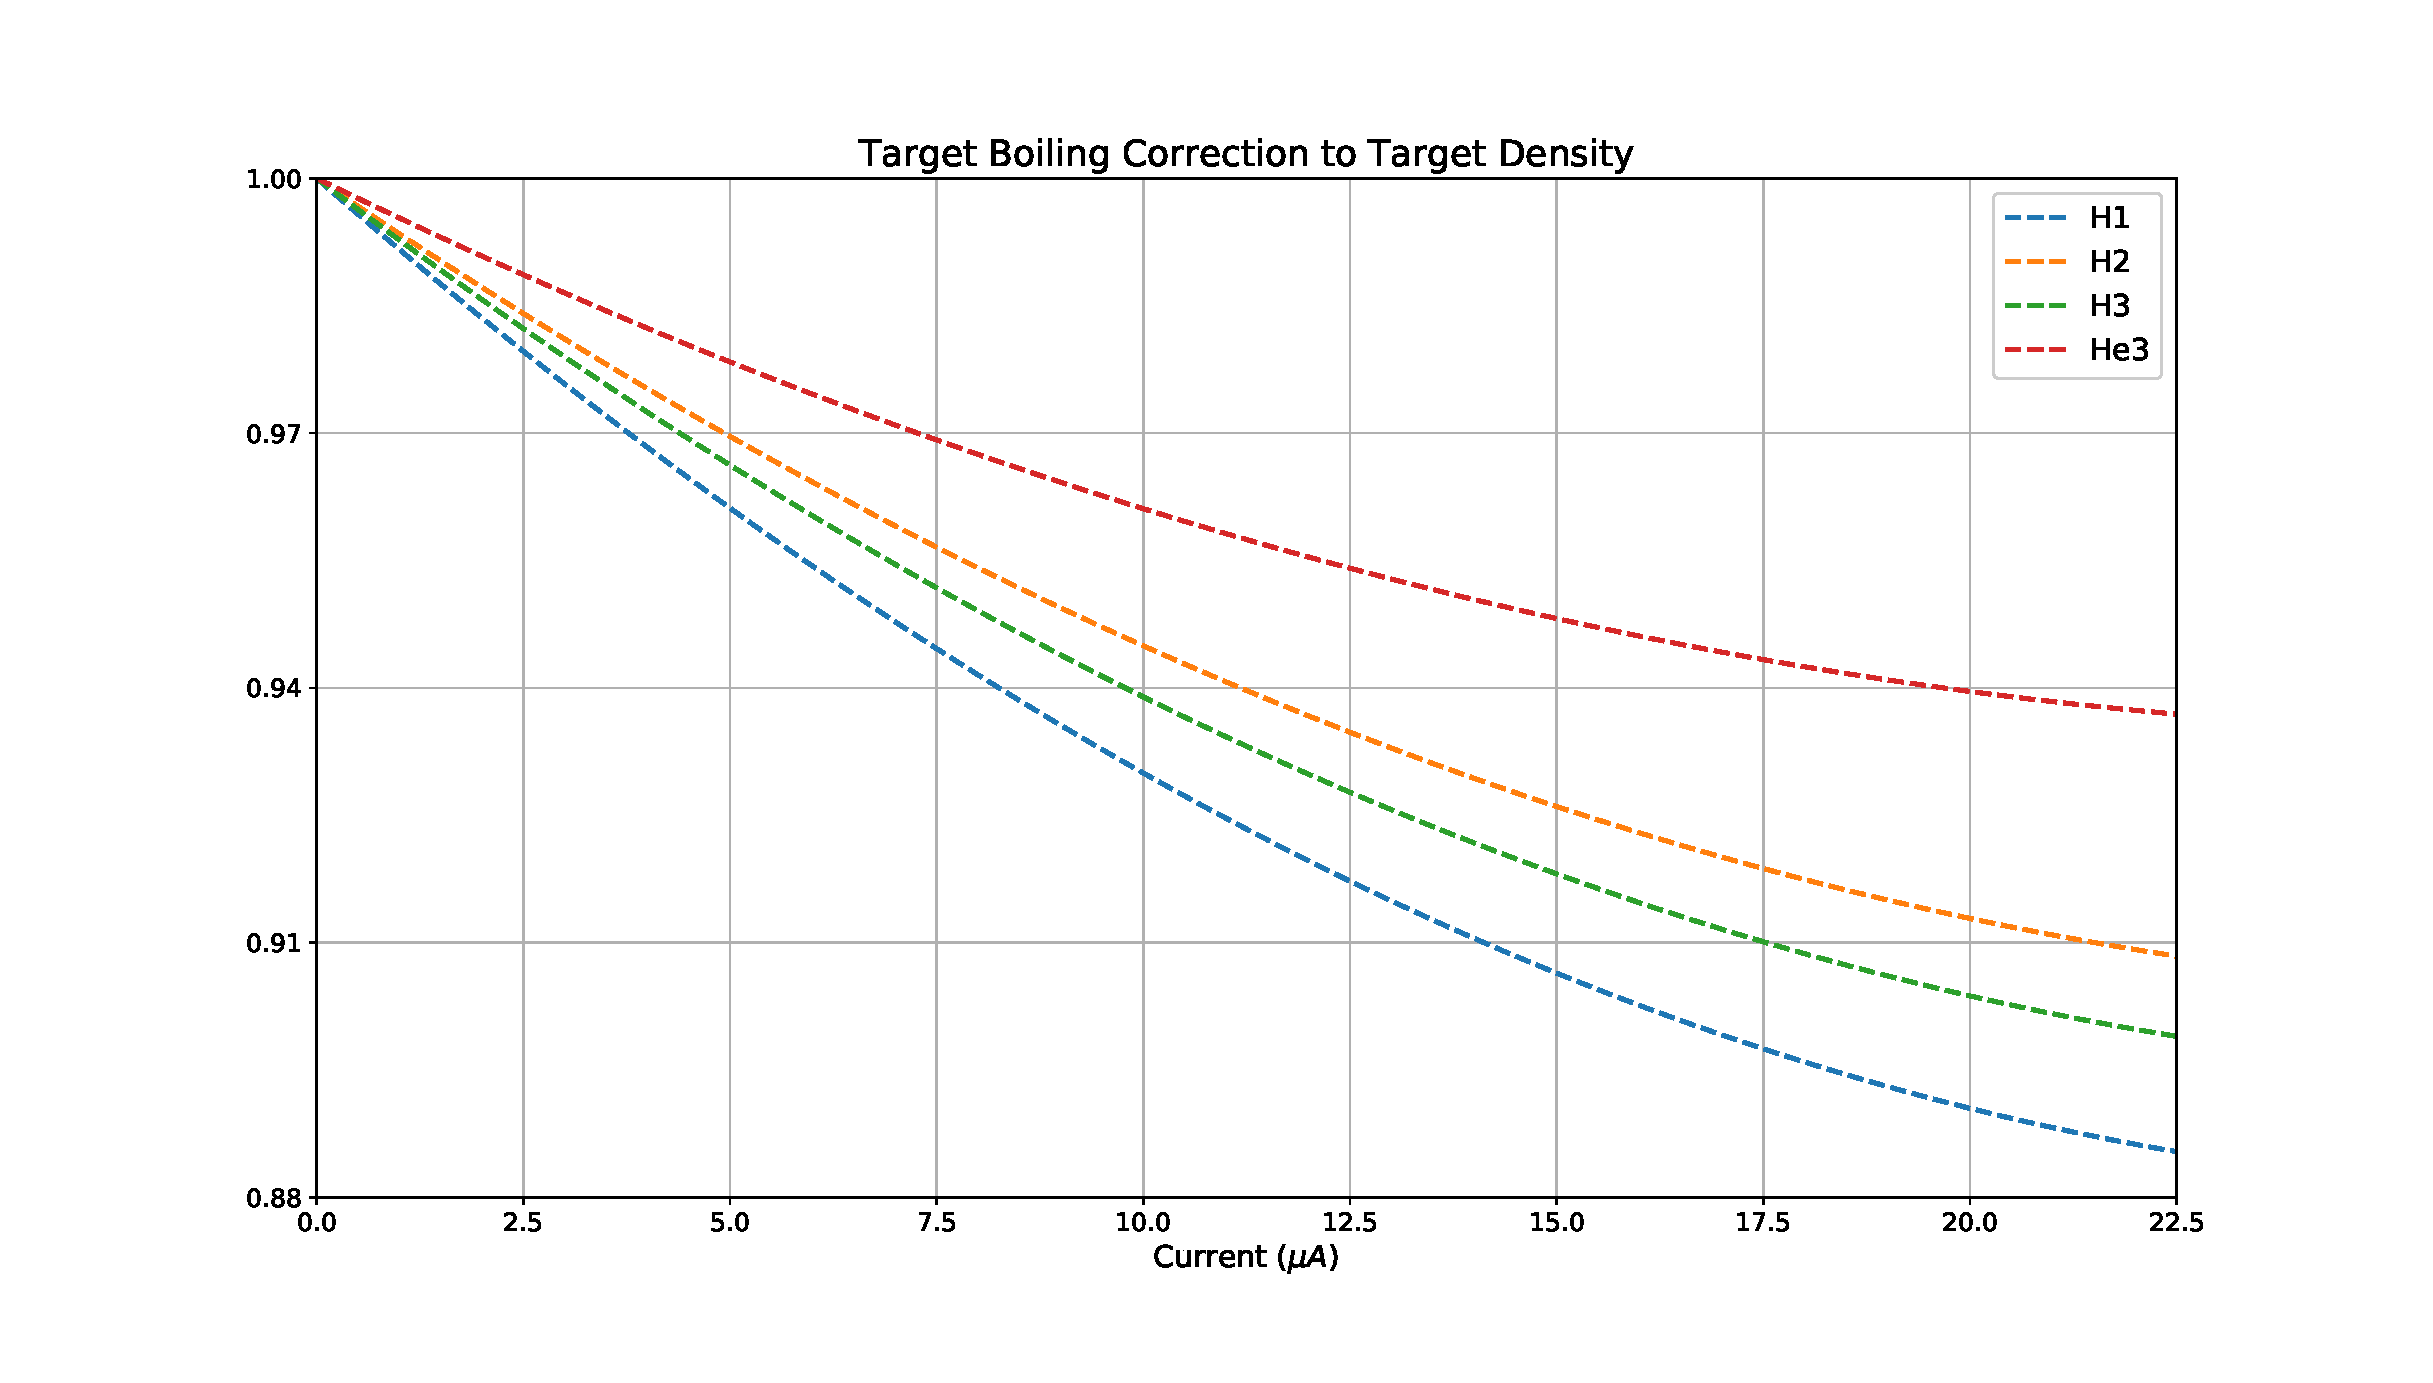
\includegraphics[width=\textwidth]{./analysis/fig/boil_cor.eps}
	\caption{Beam heating effects are manifested as a multiplicative correction to the target density}
	\label{fig:boilcor}
\end{figure}

\begin{figure}
	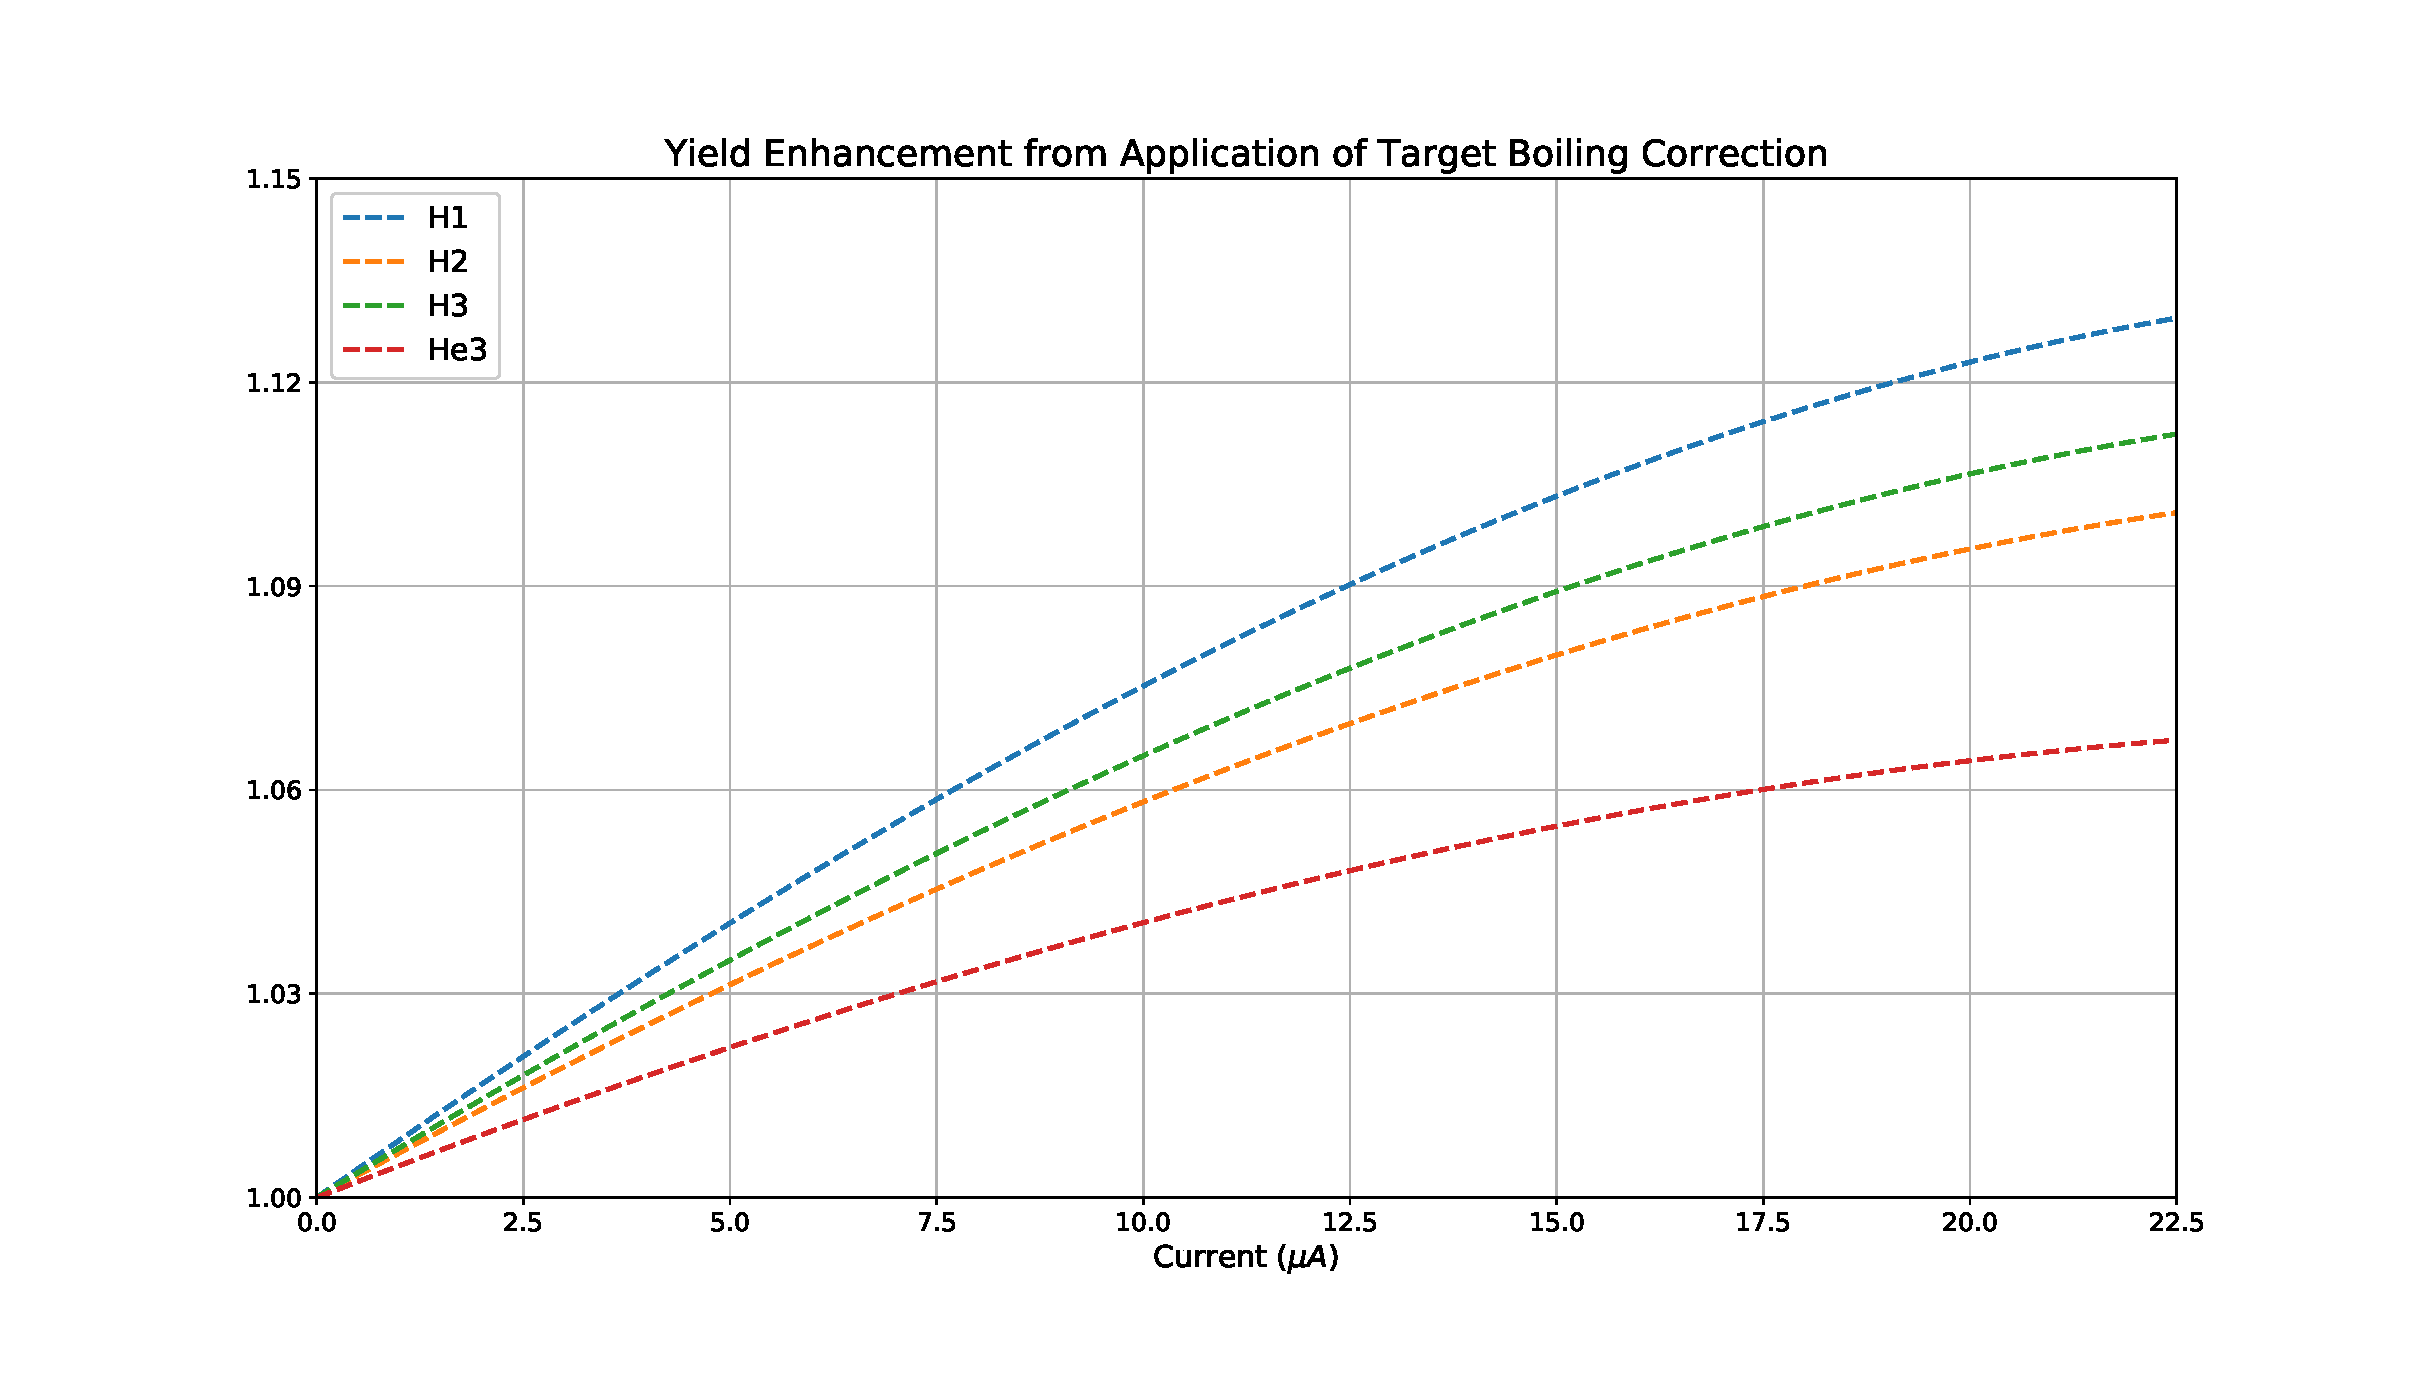
\includegraphics[width=\textwidth]{./analysis/fig/boil_yield_cor.eps}
	\caption{Target density corrections cause a multiplicative enhancement to the yield}
	\label{fig:boilyieldcor}
\end{figure}

\subsection{Target Endcap Contamination}
\label{sec:ecc}

The gas targets used in this experiment are housed in aluminum cells as described in Section \ref{sec:gas_cell}. The thickness of the aluminum greatly exceeds the thickness of the gas and will contribute background that can survive the cuts placed on the data. By quantifying this contribution, the events that originate from the cell endcaps can be subtracted from the final results.

To determine this contribution, the empty cell is used. The empty cell, being an exact replica of the gas target cells with a vacuum inside, allows us to approximately isolate the contribution of the cell walls to the data. The empty cell and the target being studied are compared by calculating the yields on a kinematic-by-kinematic basis and normalizing them by charge and endcap thickness.

The normalization to the endcaps for each target must be done in two parts. This is because each endcap is not the same thickness. When calculating the yield for a target, it is assumed that any contamination upstream (downstream) of the center of the target must originate from the upstream (downstream) endcap. The two halves are then combined to arrive at the endcap thickness normalized yield. This yield calculation only has livetime corrections applied. All cuts are applied except for target length, which is adjusted to only include events upstream (downstream) of the center of the target.

The data for the target being studied and the normalized empty target are then binned in Bjorken $x$. Dividing the empty cell data by the gas target data then gives an approximation of the fractional contribution of the cell walls to the electron data. As this correction is applied to the final results, the contamination corrections for the targets are divided by each other to create the correction to the target ratios. These results are then fit with the functional form $1\pm e^{Ax+B}$. The choice of adding or subtracting the exponential is done by determining if the correction is greater or smaller than 1. The fit function and the covariance matrix of the fit are used to apply the correction to the final results as well as determine the uncertainty contribution of this correction.

\subsection{Charge Symmetric Background Subtraction}

As an inclusive scattering experiment, we are particularly susceptible to background from charge symmetric processes from the target. To study this background we reversed the polarity of the Left HRS to take positron data at several low Bjorken x kinematics.

Measuring the positron yield allows us to determine the proportion of electron events measured that were a result of pair production. This data was subject to the same cuts that are used on the electron data. It was noted that a significant $\pi^+$ contamination occurred for the positron data. The main pion peak was fit and then subtracted from the positron data.

These data were then binned by Bjorken x and fit with an exponential. 

Somethin somethin somethin... Provide x of bin and multiply by $1-\mathrm{curve}$.

\begin{figure}
	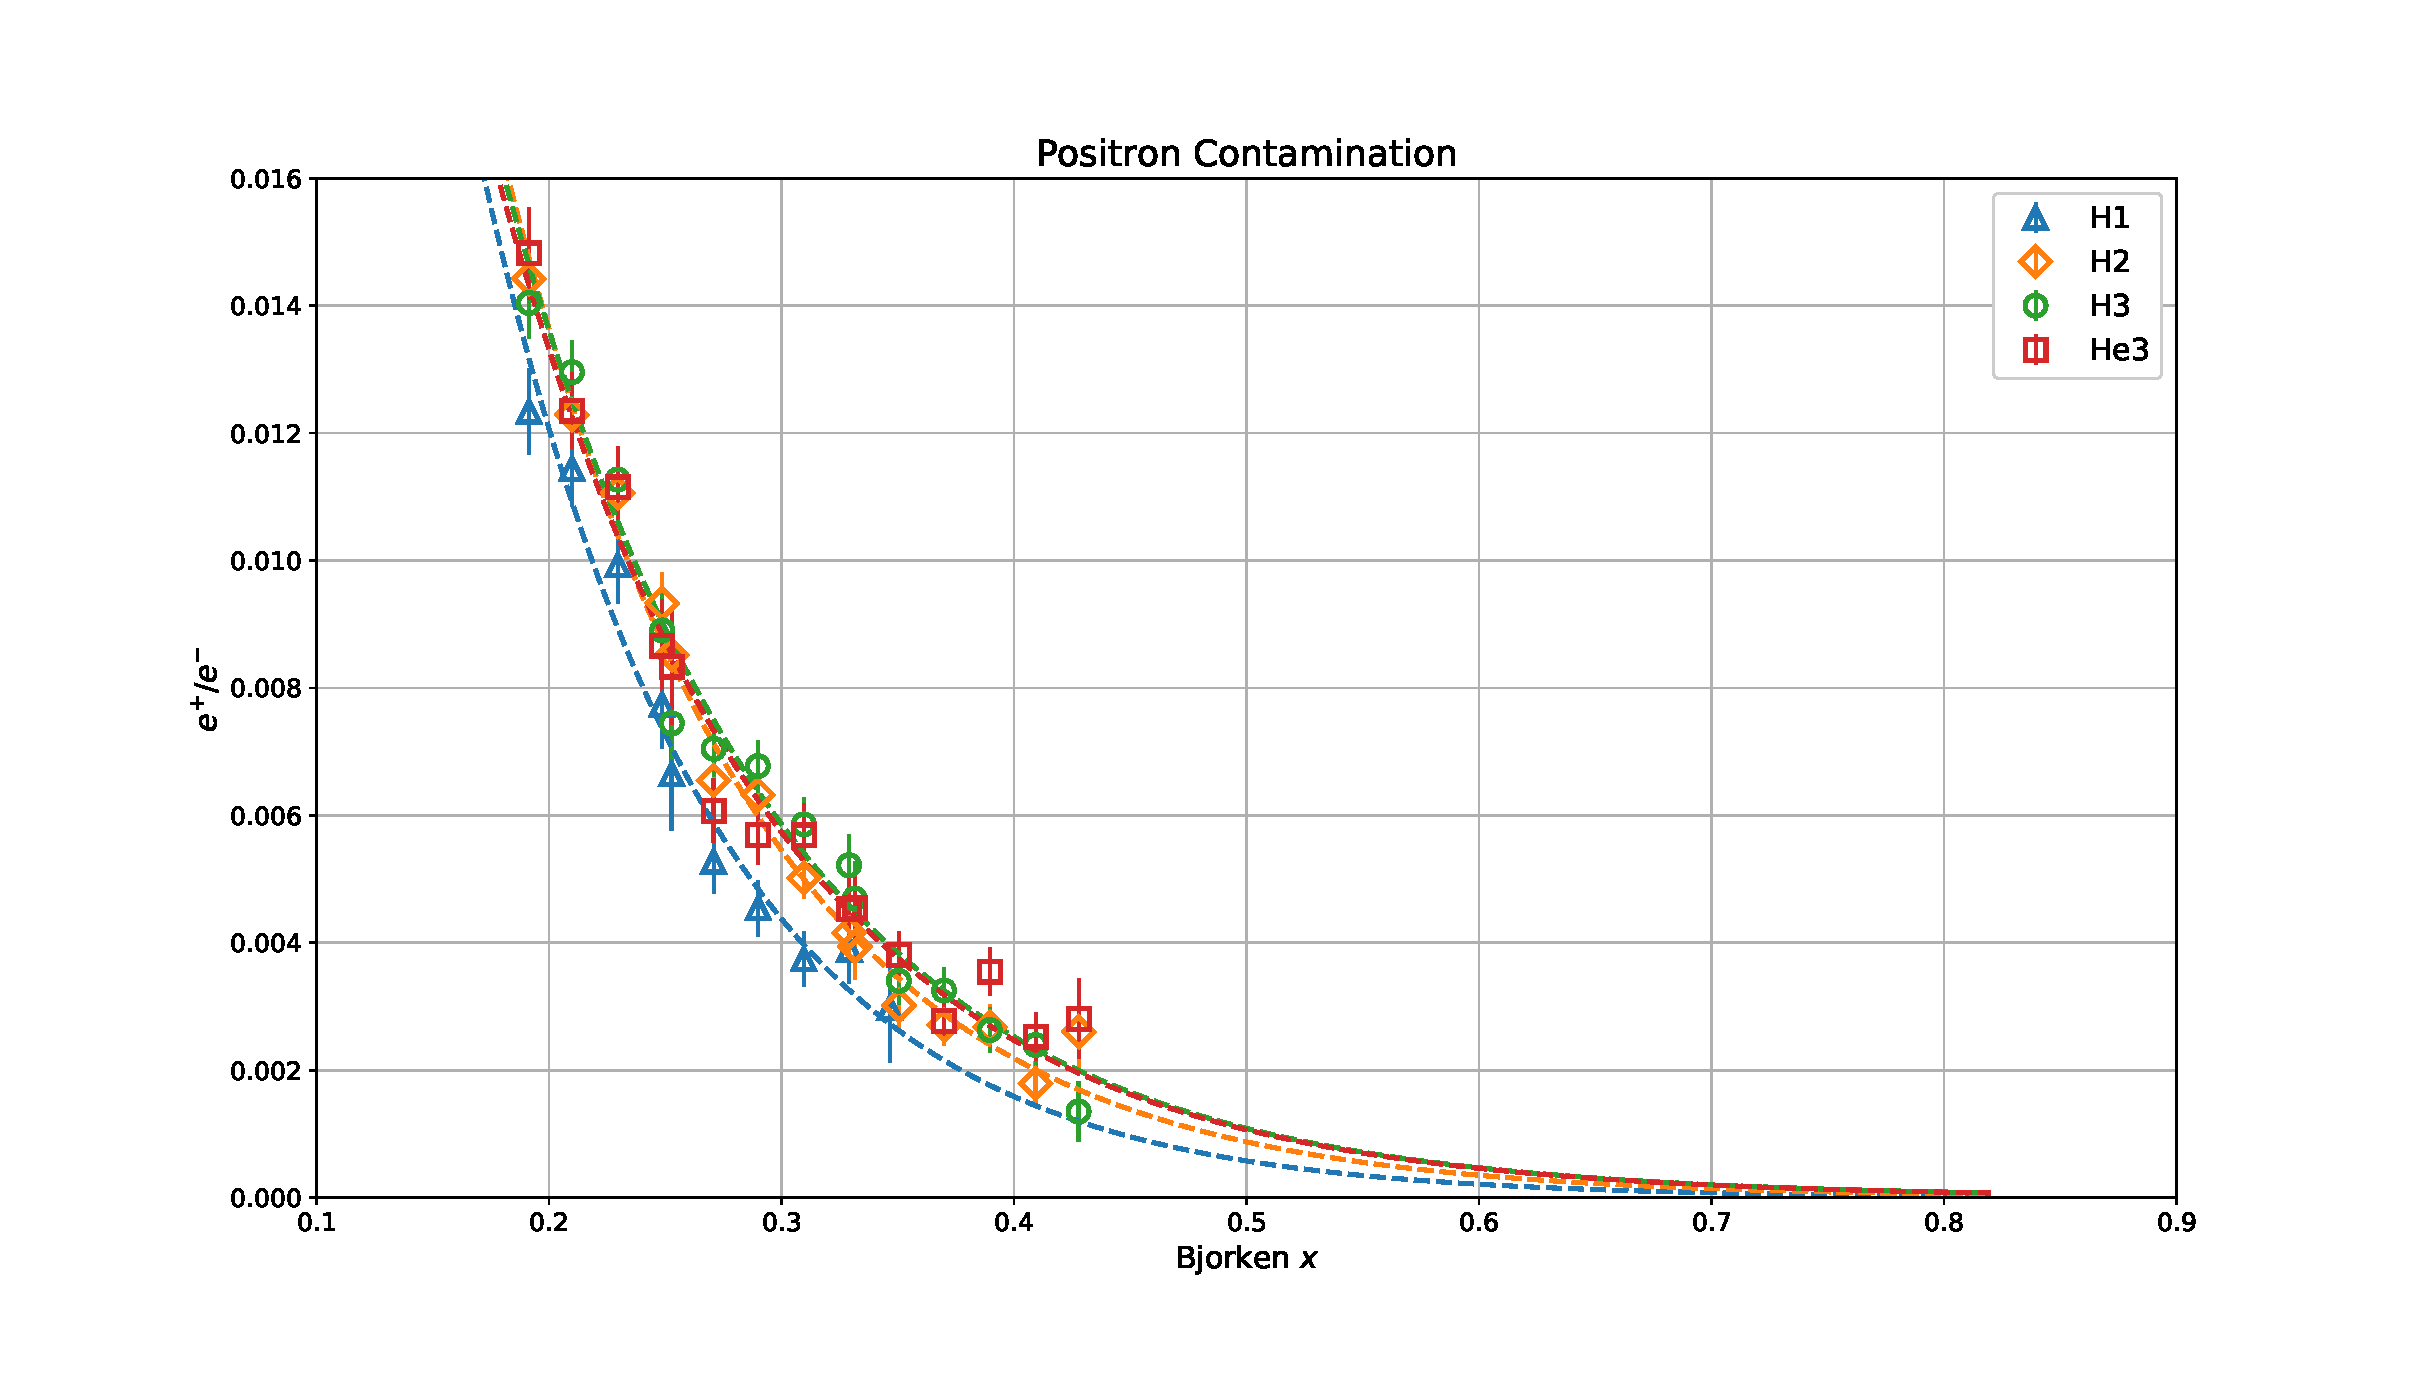
\includegraphics[width=\textwidth]{./analysis/fig/positrons.eps}
	\caption{Charge symmetric background correction}
	\label{fig:positrons}
\end{figure}

\subsection{Computer Deadtime Correction}

Our DAQ unable to continuously record data. While we can probabilistically determine the mean time spacing between events, in the real world events can deviate greatly from these means. Sometimes events will occur that are too close in time for our DAQ to record as the computer has not completed recording the previous event. Deadtime is a function of event rate; when events happen more rapidly, there is a higher chance that events will occur too closely in time to be recorded.

When deadtime is low and the number of recorded events is high, it is a reasonable assumption that the events recorded will accurately reflect the distribution of events in the ``zero-deadtime limit''. In this case correcting for the deadtime is simply done by scaling the number of events by the ``livetime'' of the experiment.

The computer livetime was measured using the Trigger Supervisor and scalers in each HRS. The trigger signals generated from detector signals are copied and sent to both the Trigger Supervisor and a scaler unit. The Trigger Supervisor is subject to the computer deadtime event loss discussed here. The scaler unit, on the other hand, simply increments a register when a trigger signal is received. The ratio of these the number of events recorded by these two systems gives a measure of the livetime of the measurement. The livetime is defined on a run-by-run basis as:

\begin{equation}
DT = \frac{\Sigma \mathrm{Triggers_{TS}}}{\Sigma \mathrm{Triggers_{Scaler}}}
\end{equation}

In an ideal world, the deadtime will be identical for all runs within a kinematic. However, the deadtime is measured on a run-by-run basis and is applied as such in order to account for any deviations from this assumption. The average deadtime for each target in each kinematic is plotted in Figure \ref{fig:deadtime}.

\begin{figure}
	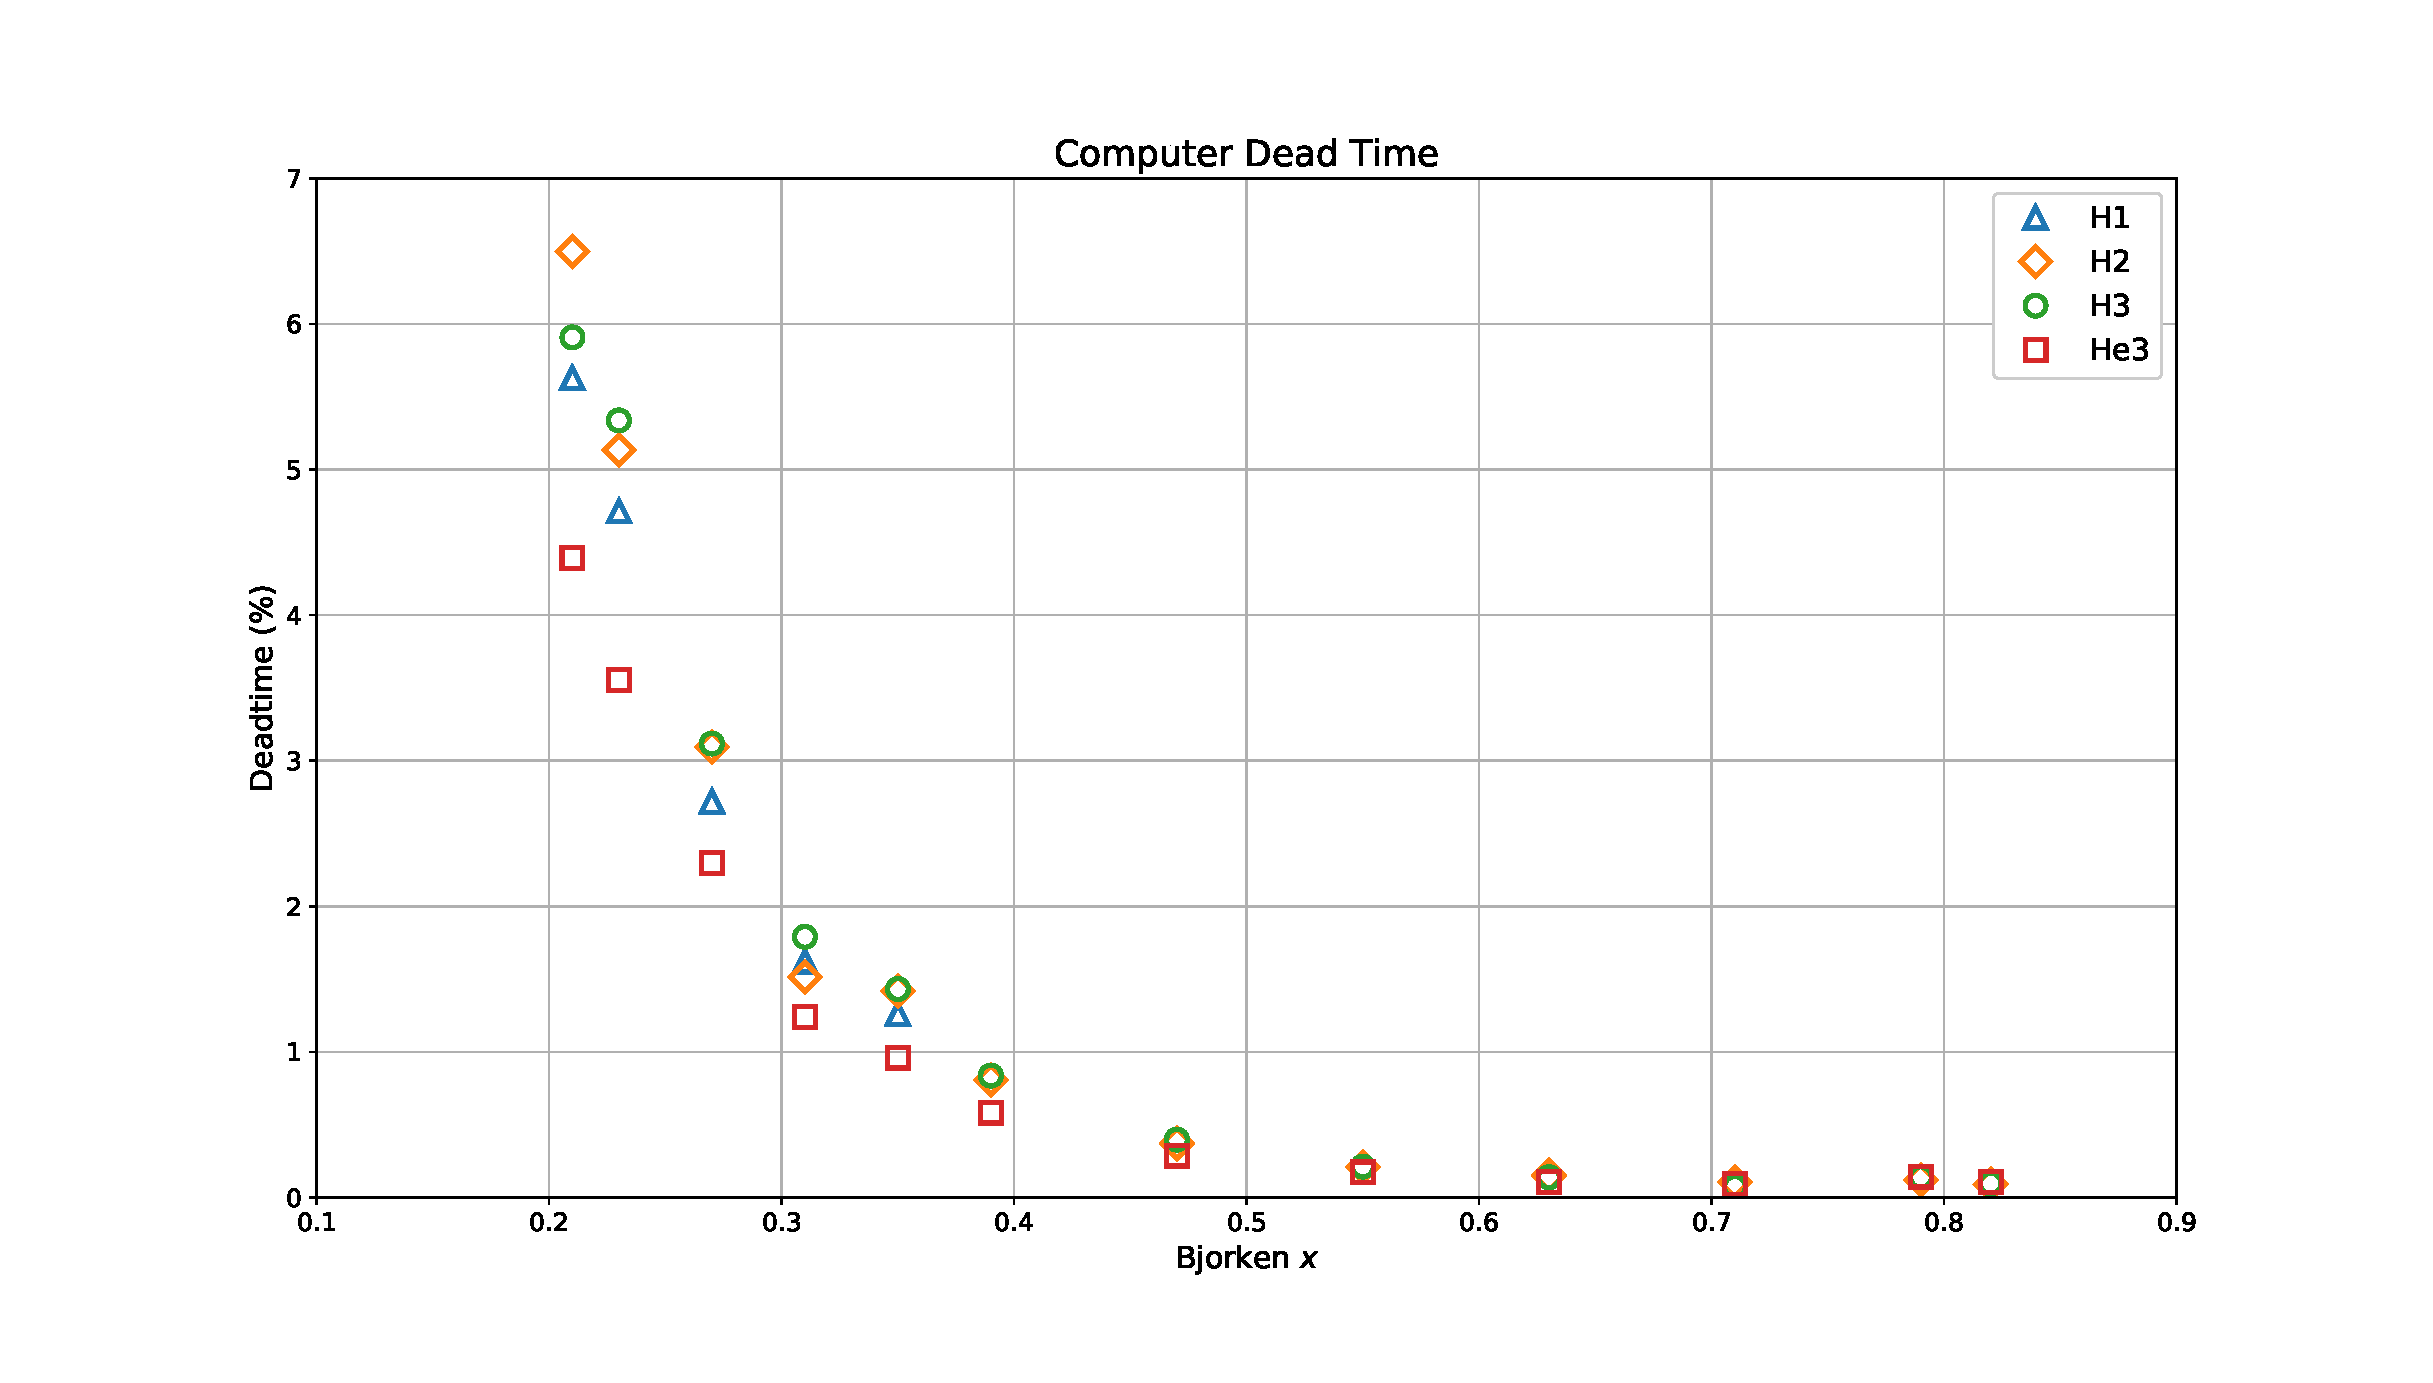
\includegraphics[width=\textwidth]{./analysis/fig/deadtime.eps}
	\caption{Deadtime per kinematic}
	\label{fig:deadtime}
\end{figure}

\subsection{Radiative Corrections}

\subsection{Isoscalar Corrections}

\subsection{Bin Centering Corrections}

The cross-section over the width of a bin is not constant. This means that the measurement does not correspond with the true cross section at the center of the bin. Using a model that matches the shape of our data well, the location of the measurement within the bin can be calculated. This is done by calculating the expectation value of the model within that bin and determining the $x$ value corresponding to this value. The expectation value is given by
\begin{equation}
	\langle f_{\rm measured}\rangle = \frac{1}{\Delta x}\int_{x_{\rm low}}^{x_{\rm high}} f\left( x \right) dx,
\end{equation}
where $f$ is a function representing the chosen model. In practice, the $x$ value does not need to be calculated if the data will be reported at the bin center. Rather, the correction is simply the ratio of the model at the bin center. This is written as
\begin{equation}
	\sigma_{\textrm{Bin Centered}} = \frac{f\left(x_{\textrm{Bin Center}}\right)}{\langle f_{\rm measured}\rangle} \sigma_{\rm measured}.
\end{equation}

This correction must be applied to both targets in the ratios. That is, the ratio must be multiplied by the correction to the numerator and divided by the correction to the denominator.\cite{wtsydp}

\subsection{Coulomb Corrections}

Corrections must be made for the effect of the charge of the target on the scattered electron. This interaction causes the $Q^2$ of the event to shift to an effective $Q^2$ value, $Q^2_{\rm eff}$. This conversion is done with the equation
\begin{equation}
	Q^2_{\rm eff} = Q^2 \left(1 + \frac{3Z\alpha\hbar c}{2RE}\right)^{2}.
\end{equation}
In this equation $R$ is the hard-sphere equivalent radius of the nucleus which is defined as $R=\left[\left(\nicefrac{5}{3}\right) \langle r^{2}\rangle\right]^{\nicefrac{1}{2}}$ where $\langle r^2\rangle$ is the root-mean-squared radius of the nucleus.\cite{coulomb}

Using $x=\frac{Q^2}{2M\nu}$, it is clear that a shift in $Q^2$ will result in a proportional shift in $x$. Using a model cross-section, the cross section is calculated at both the nominal $x$ and at $x_{\rm eff}$. As the results have been bin centered, this calculation uses a nominal $x$ at the center of the bin. This will lead to the correction
\begin{equation}
	\sigma_{\textrm{Coulomb Corrected}} = \sigma_{\rm data} \frac{\sigma_{\rm model}\left(x_{\rm eff}\right)}{\sigma_{\rm model}\left(x\right)}.
\end{equation}

This correction must be applied to both targets in the ratios that are calculated.